\chapter{向量的坐标运算~~直线与圆}

\section{向量的坐标运算}
\subsection{直角坐标系与向量的坐标}
在初中,我们已学习了平面直角坐标系,其要点如下:
选定一个长度单位,建立两条具有公共原点且互相垂直的数
轴(图5.1),通常一条为水平的数轴,称为横轴或$X$
轴,它的正向是由左到右,另一
条是和它垂直的轴称为纵轴或$Y$
轴,它的正向是从下到上。$X$
轴、$Y$轴总称为坐标轴、坐标轴的交点$O$称为坐标系的原点,这
样我们就说在平面上建立了直角
坐标系$OXY$, 这个平面就叫做
坐标平面,在坐标平面上任取一
点$P$, 过$P$引$X$轴、$Y$轴的垂线,设垂足分别是$M$、$N$, 如
果$M$在$X$轴上的坐标为$x$, $N$在$Y$轴上的坐标为$y$, 那么我
们就说$P$点的坐标是$(x,y)$, 记作$P(x,y)$, $x$称为
横坐标,$y$称为纵坐标。
\begin{figure}[htp]\centering
    \begin{minipage}[t]{0.48\textwidth}
    \centering
\begin{tikzpicture}[>=latex, scale=1]
\draw[->](-1,0)--(4,0)node[right]{$X$};
\draw[->](0,-1)--(0,3)node[right]{$Y$};
\node at (0,0)[below left]{$O$};
\draw[dashed](0,2)node[left]{$N$}--(3,2)node[right]{$P$}--(3,0)node[below]{$M$};
    \end{tikzpicture}
    \caption{}
    \end{minipage}
    \begin{minipage}[t]{0.48\textwidth}
    \centering
    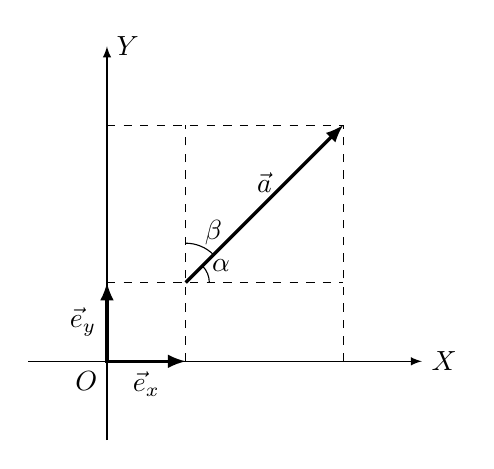
\begin{tikzpicture}[>=latex, scale=1]

\draw[->](-1,0)--(4,0)node[right]{$X$};
\draw[->](0,-1)--(0,4)node[right]{$Y$};
\draw[<->, very thick](0,1)--node[left]{$\vec{e}_y$}(0,0)--node[below]{$\vec{e}_x$}(1,0);
\draw[dashed](0,1)--(3,1);
\draw[dashed](0,3)--(3,3);
\draw[dashed](1,0)--(1,3);
\draw[dashed](3,0)--(3,3);
\draw[->, very thick](1,1)--node[above]{$\vec{a}$}(3,3);
\draw(1.3,1) arc (0:45:.3)node[right]{$\alpha$};
\draw(1,1.5) arc (90:45:.5)node[above ]{$\beta$};
\node at (0,0)[below left]{$O$};

    \end{tikzpicture}
    \caption{}
    \end{minipage}
    \end{figure}


在建立直角坐标系$OXY$的平面上(图5.2),我们
沿$X$轴与$Y$轴的正方向分别取单位向量$\vec{e}_x$、$\vec{e}_y$, 由共面向量
定理可知,对坐标平面上任一向量
$\va$, 存在唯一的有序实数偶$(a_x,a_y)$使
\begin{equation}
    \va =a_x \eX+a_y \eY
\end{equation}
$(a_x,a_y)$就叫做$\va$在直角坐标系
$OXY$上的坐标,记作
\begin{equation}
    \va=(a_x,a_y)
\end{equation}
实质上(5.2)式是(5.1)式的缩写;其中$a_x$叫做$\va$在$X$轴上
的坐标分量,$a_y$叫做$\va$在$Y$轴上的坐标分量。

\begin{blk}
    {定理} 在坐标平面上,如果$\va=(a_x,a_y)$, 则
    \begin{equation}
    \begin{split}
        a_x&=\eX\cdot \va=|\va|\cos\langle\eX,\va\rangle\\
        a_y&=\eY\cdot \va=|\va|\cos\langle\eY,\va\rangle\\
    \end{split}
    \end{equation}
\end{blk}

\begin{proof}
    已知$\va =a_x \eX+a_y \eY$,则
\[\begin{split}
   \eX\cdot \va&=\eX\cdot (a_x\eX+a_y\eY)=a_x\eX\cdot \eX+a_y\eX\cdot \eY\\
   \eY\cdot \va&=\eY\cdot (a_x\eX+a_y\eY)=a_x\eY\cdot \eX+a_y\eY\cdot \eY\\ 
\end{split}\]
由于$\eX,\eY$是单位向量,且$\eX\bot \eY$, 所以,
\[\eX\cdot \eX=\eY\cdot \eY=1,\qquad \eX\cdot \eY=\eY\cdot \eX=0\]
于是得到
\[    \begin{split}
    a_x&=\eX\cdot \va=|\va|\cos\langle\eX,\va\rangle\\
    a_y&=\eY\cdot \va=|\va|\cos\langle\eY,\va\rangle\\
\end{split}\]
\end{proof}

这个定理说的是,\textbf{向量$\va$在$X$轴和$Y$轴上的坐标分量分
别是$\va$在坐标轴上的垂直投影量}。

显然,$\vec{o}=(0, 0)$, $\eX=(1, 0)$, $\eY=(0, 1)$. 令$\expval{\eX,\vec{a}}=\alpha$, $\expval{\eY,\vec{a}}=\beta$,$\alpha,\beta$一起决定了$\vec{a}$的方向,$\alpha,\beta$叫做$\vec{a}$的\textbf{方向角},$\cos\alpha$, $\cos\beta$叫做$\vec{a}$的\textbf{方向余弦},上述定理表达了向量的长度、方向与它的坐标之间的关系,甚为重要,请同学要把它牢牢记住。

如果在坐标平面上(图5.3),以$O$为起点引
$\Vec{OA}=\vec{a}$, 则$A$点的位置被$\vec{a}$所唯一确定,这时,我们称$\Vec{OA}$为点$A$的\textbf{位置向量}。换句话说,$A$点的位置向量也就是确定$A$点相对于原点位置的向量。设$\Vec{OP}=x\eX+y\eY$,则$\Vec{OP}$的坐标$(x,y)$也就是$P$点的坐标;反之,$P$点的坐标$(x,y)$也就是位置向量$\Vec{OP}$的坐标。由此可见,给
定了原点$O$和两个互相垂直的单位向量$\eX,\eY$, 坐标系也就完全确定了,因而,坐标系$OXY$也可用$[O:\; \eX,\eY]$来表示,$\eX,\eY$叫做坐标系的\textbf{基向量}。

\begin{figure}[htp]
    \centering
    \begin{minipage}[t]{0.48\textwidth}
    \centering
    \begin{tikzpicture}[>=latex, scale=1]
      \draw[->](-1,0)--(4,0)node[right]{$X$};
\draw[->](0,-1)--(0,3)node[right]{$Y$};
\node at (0,0)[below left]{$O$};
\draw[very thick,->](0,0)--node[above]{$\vec{a}$}(3.5,2)node[right]{$A$};
\draw[thick,->](0,0)--(1,0)node[below]{$\eX$};
\draw[thick,->](0,0)--(0,1)node[left]{$\eY$};
    \end{tikzpicture}
    \caption{}
    \end{minipage}
    \begin{minipage}[t]{0.48\textwidth}
    \centering
    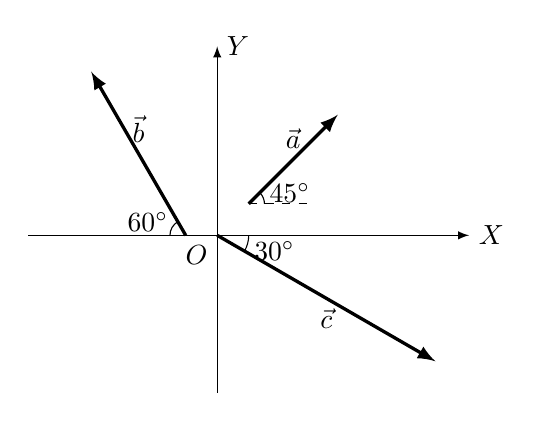
\begin{tikzpicture}[>=latex, scale=.8]
      \draw[->](-3,0)--(4,0)node[right]{$X$};
\draw[->](0,-2.5)--(0,3)node[right]{$Y$};
\node at (0,0)[below left]{$O$};
\draw[very thick,->](.5,0.5)--node[above]{$\vec{a}$}+(45:2);
\draw[very thick,->](-.5,0)--node[above]{$\vec{b}$}+(120:3);
\draw[very thick,->](0,0)--node[below]{$\vec{c}$}(-30:4);
\draw[dashed](.5,.5)--(1.5,.5);
\draw(.75,.5) arc (0:45:.25)node[right]{$45^{\circ}$};
\draw(-.75,0) arc (180:120:.25)node[left]{$60^{\circ}$};
\draw(.5,0) arc (0:-30:.5)node[right]{$30^{\circ}$};
    \end{tikzpicture}
    \caption{}
    \end{minipage}
  \end{figure}

为了方便,在本书中我们约定,当点用大写字母标记时,它相对于原点的位置向量用相应的小写字母来标记,例
如$P$点的位置向量记为$\vec{p}$, $A$点的位置向量记为$\vec{a}$等等。

\begin{example}
    向量$\vec{a}$、$\vec{b}$、$\vec{c}$的方向与绝对值如图5.4所示,求$\vec{a}$、$\vec{b}$、$\vec{c}$的坐标。
\end{example}

\begin{solution}
设$\vec{a}=(a_x,a_y)$, $\vec{b}=(b_x,b_y)$, $\vec{c}=(c_x,c_y)$, 因此:
\[\begin{split}
a_x&=\eX\cdot \vec{a}=|\vec{a}|\cos\expval{\eX,\vec{a}}=2\cos 45^{\circ}=\sqrt{2}\\
a_y&=|\vec{a}|\cos\expval{\eY,\vec{a}}=2\cos 45^{\circ}=\sqrt{2}\\
\end{split}\]
$\therefore\quad \vec{a}=\left(\sqrt{2},\sqrt{2}\right)$
\[\begin{split}
    b_x&=|\vec{b}|\cos\expval{\eX,\vec{b}}=3\cos (180^{\circ}-60^{\circ})=-3\cos 60^{\circ}=-\frac{3}{2}\\
b_y&=|\vec{b}|\cos\expval{\eY,\vec{b}}=3\cos (90^{\circ}-60^{\circ})=3\cos30^{\circ}=\frac{3}{2}\sqrt{3}\\
\end{split}\]
$\therefore\quad \vec{b}=\left(-\frac{3}{2},\frac{3}{2}\sqrt{3}\right)$
\[\begin{split}
c_x&=|\vec{c}|\cos\expval{\eX,\vec{c}}=4\cos 30^{\circ}=2\sqrt{3}\\
c_y&=|\vec{c}|\cos\expval{\eY,\vec{c}}=4\cos (30^{\circ}+90^{\circ})=-4\sin 30^{\circ}=-2\\
\end{split}\]
$\therefore\quad \vec{c}=\left(2\sqrt{3},-2\right)$
\end{solution}

\begin{ex}
\begin{enumerate}
    \item 求图中向量的坐标。
    \item 已知$A(4, 2)$, $B(-2, 5)$, $C(-4,-3)$, $D(4,-4)$. 试用基向量$\eX,\eY$表示它们相对于原点的位置向量。
    \item 已知$\Vec{OA}=(3,-1)$, $\Vec{OB}=(2, 3)$. 试写出$A$、$B$两点的坐标。
\end{enumerate}
\end{ex}

\begin{figure}[htp]
    \centering
    \begin{minipage}[t]{0.48\textwidth}
    \centering
    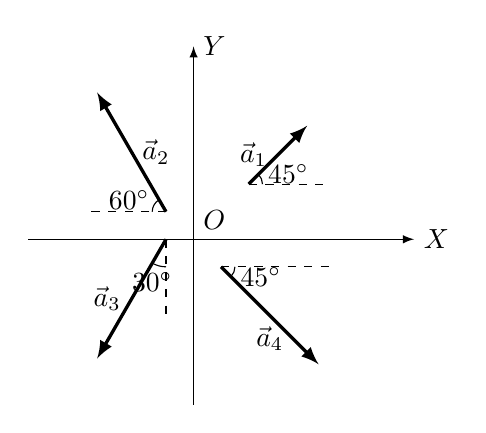
\begin{tikzpicture}[>=latex, scale=.7]
\draw[->](-3,0)--(4,0)node[right]{$X$};
\draw[->](0,-3)--(0,3.5)node[right]{$Y$};
\node at (0,0)[above right]{$O$};
\draw[very thick,->](1,1)--node[left]{$\vec{a}_1$}+(45:1.5);
\draw[very thick,->](-.5,0.5)--node[right]{$\vec{a}_2$}+(120:2.5);
\draw[very thick,->](-.5,0)--node[left]{$\vec{a}_3$}+(-120:2.5);
\draw[very thick,->](.5,-.5)--node[below]{$\vec{a}_4$}+(-45:2.5);
\draw[dashed](1,1)--(2.5,1);
\draw[dashed](-.5,0.5)--(-2,.5);
\draw[dashed](-.5,0)--(-.5,-1.5);
\draw[dashed](.5,-.5)--(2.5,-.5);

\draw(1.25,1) arc (0:45:.25)node[right]{$45^{\circ}$};
\draw(-.75,0.5) arc (180:120:.25)node[left]{$60^{\circ}$};
\draw(-.5,-.5) arc (-90:-120:.5)node[below]{$30^{\circ}$};
\draw(.75,-.5) arc (0:-45:.25)node[right]{$45^{\circ}$};
    \end{tikzpicture}
    \caption*{第1题}
    \end{minipage}
    \begin{minipage}[t]{0.48\textwidth}
    \centering
    \begin{tikzpicture}[>=latex, scale=.4]
\draw[->](-5,0)--(5,0)node[right]{$X$};
\draw[->](0,-5)--(0,6)node[right]{$Y$};
\node at (0,0)[below left]{$O$};
\tkzDefPoints{4/2/A, -2/5/B, -4/-3/C, 4/-4/D, 0/0/O}
\tkzDrawSegments[very thick,->](O,A O,B O,C O,D)
\tkzAutoLabelPoints[center=O](A,B,C,D)
    \end{tikzpicture}
    \caption*{第2题}
    \end{minipage}
  \end{figure}

\subsection{用向量坐标进行向量运算}
已知向量$\vec{a}=(a_x,a_y)$, $\vec{b}=(b_x,b_y)$,则
\[\vec{a}+\vec{b}= (a_x\eX+a_y\eY) +(b_x\eX+b_y\eY)= (a_x+b_x) \eX+ (a_y+b_y) \eY\]
即
\[\vec{a}+\vec{b}=(a_x,a_y)+(b_x,b_y)=(a_x+b_x,a_y+b_y) \]
同样可证:
\[\vec{a}-\vec{b}= (a_x, a_y ) -(b_x,b_y)=(a_x-b_x,a_y-b_y)\]

这就是说\textbf{向量的和与差的坐标等于各向量相应坐标的和与差}。

已知$\vec{a}=(a_x,a_y)$和一实数$\lambda$,则
\[\lambda a=\lambda (a_x\eX+a_y\eY) = \lambda a_x\eX+\lambda a_y\eY\]
即:$\lambda\vec{a}=\lambda (a_x ,a_y) = (\lambda a_x,\lambda a_y)$.

这就是说\textbf{向量倍积的坐标等于该向量相应的坐标与倍数的乘积}。

已知$\vec{a}=(a_x,a_y)$, $\vec{b}=(b_x,b_y)$, 则
\[\begin{split}
    \vec{a}\cdot \vec{b}&=(a_x\eX+a_y\eY)\cdot (b_x\eX+b_y\eY)\\
    &=a_xb_x\eX\cdot \eX+a_xb_y\eY\cdot \eX+a_yb_x\eY\eX+a_yb_y\eY\cdot \eY
\end{split}\]
由于$\eX\cdot \eX=\eY\cdot \eY=1$, $\eX\cdot \eY=\eY\cdot \eX=0$,所以
\[\vec{a}\cdot \vec{b}=(a_x,a_y)\cdot (b_x,b_y)=a_xb_x+a_yb_y\]













































































































































































\begin{ex}
\begin{enumerate}
    \item 已知
 \begin{enumerate}
    \item $\vec{a}=(3,-4),\quad \vec{b}=(2,-7)$;
    \item $\vec{a}=(-5,-6),\quad \vec{b}=(4,-9)$.
\end{enumerate}   
    求由$\vec{a},\vec{b}$作邻边向量张成的平行四边形的面积。
    
    \item 已知$A(2, 3)$, $B(-7, 5)$, $C(3,-5)$,求
    $\triangle ABC$的面积。
    \item  已知$A(-10,-8)$, $B(9,-3)$, $C(2, 11)$, 求
    $\triangle ABC$的面积。
    \item 说明$\begin{vmatrix}
       a_x&a_y\\b_x&b_y 
    \end{vmatrix}=-\begin{vmatrix}
        \b_x&b_y \\a_x&a_y
    \end{vmatrix}$
    的几何意义。
    \item 说明$\begin{vmatrix}
        a_x&a_y\\a_x+b_x&a_y+b_y 
     \end{vmatrix}=\begin{vmatrix}
         a_x&a_y \\\b_x&b_y
     \end{vmatrix}$的几何意义。
\end{enumerate}
\end{ex}

\subsection*{习题5.1}
\begin{enumerate}
    \item 在$X$轴上的点,它的纵坐标都等于什么?在$Y$轴上的点,它的横坐标都等于什么?
    \item 在坐标平面上,已知边长为$a$的正方形$ABCD$, $A$与原点重合,$\Vec{AB}$, $\Vec{AD}$的方向分别与$X$轴和$Y$轴的正方向一致,求四个顶点的坐标。
    \item 分别求点$(a,b)$关于$X$轴、$Y$轴的对称点的坐标。
    \item 已知$|\Vec{OA}|=7$、$|\Vec{OB}|=6$, 点$A$在第四象限,点$B$在第二象限,且$\expval{\Vec{OA},\eX}=45^{\circ}$, $\expval{\Vec{OB},\eY}=30^{\circ}$. 求$A$点、$B$点的坐标。
    \item $\parallelogram{ABCD}$中的$\Vec{AB}=8$, $\Vec{AD}=5$, $\angle A=60^{\circ}$,如果取$A$作原点,$X$轴正方向与$\Vec{AB}$同向,$C$点所在的象
    限为第一象限,求它各顶点的坐标。
    \item 已知
\begin{multicols}{2}
\begin{enumerate}
    \item $A(-3, 4),\quad B(2,-5)$; 
    \item $A(2,-1),\quad B(-4, 3)$
\end{enumerate}
\end{multicols}
    求$\Vec{AB}$的坐标。
    
\item 已知$|\vec{a}|=12$, $\expval{\eX,\vec{a}}=30^{\circ}$, $\expval{\eY,\vec{a}}=120^{\circ}$, 
    求$\vec{a}$的坐标。
    
    \item 建立坐标系$[O:\; \eX,\eY]$, 画出下列各向量。
\begin{multicols}{3}
\begin{enumerate}
    \item $\eX=(1,0)$
    \item $\eY=(0,1)$
    \item $\vec{a}=(-1,1)$
    \item $\vec{b}=(0,2)$
    \item $\vec{c}=(-2,0)$
    \item $\vec{d}=(0,-2)$
    \item $\vec{f}=(-1,-3)$
\end{enumerate}
\end{multicols}

\item 问平行于$X$轴的向量与平行于$Y$轴的向量的坐标各有什么特点。
\item 证明$A,B,C$三点共线。
\begin{enumerate}
    \item $A (2, 1) ,\quad  B (0, 5) ,\quad  C (4, -3)$
    \item $A (-1, 0) ,\quad  B (1, -2) ,\quad  C (3, -4)$
\end{enumerate}
\item 已知$\parallelogram{ABCD}$, $\overline{AC}$, $\overline{BD}$相交于$P$, 且$A(-1, 2)$, $B(3, 0)$, $P(0, 2)$, 求$B,C$两顶点的坐标。
\item 求证$\vec{m}=(-2, 3)$, $\vec{n}=(2,-3)$与$\vec{a}=(3, 2)$垂直并作图验证。
\item 已知$\vec{a}=(2,-1)$, $\vec{b}=(-1, 1)$, 求$\vec{a}+\vec{b}$, $\vec{a}-\vec{b}$, $\vec{a}\cdot \vec{b}$, 
$\left(3\vec{a}-2\vec{b}\right)\cdot\left(\vec{a}+4\vec{b}\right)$.
\item 已知$\vec{a}=(1, 2)$, $\vec{b}=(3, 1)$. 在坐标平面上
画出$\vec{a}+\vec{b}$, $\vec{a}+2\vec{b}$, $\vec{a}+3\vec{b}$, $\vec{a}-2\vec{b}$, $\vec{a}-3\vec{b}$.

\item 已知$A(1, 3)$, $B(2,-1)$, $C(4,k)$, 问$k$为何值时,$\triangle ABC$是等腰三角形。
\item 已知$A(1, 1)$, $B(2,-1)$. 如果$\triangle ABC$是
等边三角形,且$A,B,C$按逆时针顺序排列,求顶点$C$的坐标。
\item 已知$|\vec{a}| = 2$, $\vec{b}=(\sqrt{3}, 1)$, $\vec{a}$到$\vec{b}$的旋转角为$60^{\circ}$, 求$\vec{a}$的坐标。
\item 已知$A(2, 3)$, $B(-1, 0)$, $C$点在$\overline{AB}$的垂直平
分线上,且和$\overline{AB}$的距离是$\overline{AB}$长的一半,求$C$点的坐标。
\item 已知正方形$ABCD$, $A(0,-1)$, $B(-2, 1)$, 
$A$、$B$、$C$、$D$四点
\begin{multicols}{2}
\begin{enumerate}
    \item 按顺时针顺序排列;
    \item 按逆时针顺序排列。
\end{enumerate}
\end{multicols}
求$C$点的坐标。
\item 已知正六边形$ABCDEF$, $A$、$B$、$C$、$D$、$E$、$F$
成逆时针方向排列,$A(1, 1)$, $B(-2, 3)$, 求顶点$C$、$D$、$E$、$F$的坐标。
\item 计算由下列各对向量张成的平行四边形的面积。
\begin{enumerate}
    \item $\vec{a}= (3, -2) ,\qquad \vec{b}= (5, 1)$
    \item $\vec{a}= (1, 2) ,\qquad \vec{b}= (-1, 2) $
    \item $\vec{a}= (-2, 3) ,\qquad \vec{b}= (-3, 4) $
\end{enumerate}
\end{enumerate}

\section{直线方程}
一个关于$x$、$y$的二元方程总可写为
\begin{equation}\label{lin_eq}
 F (x,y) =0   
\end{equation}
的形式。例如$x+y-3=0$, $y-x^2=0$, $x^2+2xy-y^2-3=0$等.设满足方程(\ref{lin_eq})的所有实数偶$(x,y)$的集合用$A$表示,则$A$可描述为
\[A= \{ (x,y) |F (x,y) =0\} \]
对$A$中的每一个有序实数偶$(x,y)$, 在坐标平面上,唯一确定了一个点$P(x,y)$. 这样,$A$中的所有元素就对应着平面上的一个点集$B$. $B$可描述为
\[B= \{P (x,y) |F (x,y) =0\}\]

点集$B$叫做方程$F(x,y)=0$的图象或轨迹,而$F(x,y)=0$又叫做轨迹方程。例如:方程$y-x=0$的所有解集
\[\{ (x,y) |y-x=0\}\]
对应着坐标平面上点的轨迹
\[\{P (x,y) |y-x=0\} \]
是第1、第3象限的角平分线。方程$y-x^2=0$的解集
\[\{ (x,y) |y-x^2=0\}\]
所对应的点轨迹
\[\{P (x,y) |y-x^2=0\}\]
是坐标平面上一条抛物线。

如果我们要确定某个点集是某个二元方程$F(x,y)=0$的轨迹,或方程$F(x,y)=0$是某个点集的方程,显然必
须证明以下两条。
\begin{enumerate}
    \item $(x,y)\in A\quad \Rightarrow\quad P(x,y)\in B$
    \item $P (x,y) \in B\quad \Rightarrow\quad  (x,y) \in A$
\end{enumerate}
第一条保证满足方程$F(x,y)=0$的实数偶所对应的点一定在轨迹$B$上,第二条保证在轨迹$B$上的点的坐标一定满足方程$F(x,y)=0$.

设$A= \{P (x,y) |F (x,y) =0\}$, $B= \{P (x,y) |G (x,y) =0\}$. 
$A,B$是两个轨迹。由定义可知,求$A\cap B$, 即求$A$与$B$的交集,与求联立方程
\[\begin{cases}
   F (x,y) =0\\
   G (x,y) =0 
\end{cases}\]
的解集,在解析几何中是同一件事。

这一节我们首先研究直线方程。

































































\subsection*{习题5.3}
\begin{enumerate}

\item 求通过点$(0,0)$、$(a,0)$、$(0,a)$的圆的方程。
\item 求下列每个圆的圆心和半径。
\begin{enumerate}
    \item $(x-a)(x-b)+(y-c)(y-d)=0$
    \item $(x+y+a)^2+(x-y-a)^2=8a^2$
\end{enumerate}

\item 已知$A(2,-1)$, $B(2,3)$, $C(4,-1)$, 求
$\triangle ABC$的外接圆的圆心和半径。
\item 证明通过$A(a,c)$, $B(b,c)$和$C(b,d)$的圆的方
程是$(x-a)(x-b)+(y-c)(y-d)=0$.
\item $P$是圆心在$A(a,b)$且通过原点的圆上的一动点,求
证$\triangle OAP$重心的轨迹方程是
\[3(x^2+y^2)-4ax-4by+a^2+b^2=0\]
\item 证明$A(6,3)$、$B(5,4)$、$C(1,-2)$和$D(6,
-1)$四点共圆。
\item 一动点到原点的距离的平方是它到定直线$x=1$距离的
4倍,求证这动点的轨迹是点圆$(2,0)$或圆$(x+2)^2
+y^2=8$.
\item 已知三角形由直线$x=2$, $y=4$和$4x+3y=32$围成,
求这三角形内切圆的方程。
\item 已知$A(x_1,y_1)$, $B(x_2,y_2)$, $C(x_3,y_3)$, 一动点
$P(x,y)$使$\overline{AP}^2+\overline{BP}^2+\overline{CP}^2=$常数,证明$P$点的
轨迹是一个圆且它的圆心是$\triangle ABC$的重心。
\item 已知$A(2a,0)$, $C(0,2a)$, $\overline{AC}$是正方形$OABC$的
对角线,一动点$P(x,y)$到这正方形四边距离的平方和
等于$12a^2$, 证明$P$点的轨迹是圆心在$(a,a)$, 半径是$2a$
的圆。
\item 已知$A(3,7)$, $B(-1,5)$, 动点$P(x,y)$使
$\overline{AP}^2+\overline{BP}^2=82$, 证明$P$点的轨迹是半径等于6的圆。
\item 已知$A(3,7)$, $B(1,-1)$, 动点$P$使$\overline{AP}=3\overline{BP}$. 
证明$P$点的轨迹是一个圆且这圆在Y轴上截出的弦长等
于6.
\item 已知$OC$是圆$x^2+y^2-2ax=0$的一条弦,直线$OC$的
斜率是$m$, 求证以$OC$作直径圆的方程是
\[(1+m^2)(x^2+y^2)-2a(x+my)=0\]
\item 如果$a,b$是常数,$\theta$是一动角,求证两直线$x\cos\theta+
y\sin\theta=a$与$x\cos\theta-y\sin\theta=b$的交点的轨迹是一个圆
圆心在原点.半径等于$\sqrt{a^2+b^2}$.
\item 已知一圆与$Y$轴相切于$A(0,-3)$且半径$r=2$, 求
此圆的方程。
\item 已知一圆与两坐标轴相切且通过$A(2,9)$, 求它的方
程。
\item 已知一圆与$X$轴相切于$(5,0)$且在$Y$轴上截出的弦长是10, 求此圆的方程。
\item 求圆:$x^2+y^2=25$与平行线系$x+5y+\lambda=0,\quad (\lambda\in\mathbb{R})$
相交所截弦中点的轨迹。
\item 求二圆$x^2-12x+y^2-10y+52=0$, $x^2+18x+y^2+
20y+60=0$的圆心距及原点到连心线的距离。
\item 在直线系$y-7+\lambda(x+1)=0$中,求与圆$x^2+y^2=2$
相切之直线。
\item 求通过点$(5,-2)$且与已知直线$3x-y-1=0$相切于
点$(1,2)$的圆的方程。
\end{enumerate}

\section*{复习题五}
\begin{enumerate}
    \item 一个正六边形边长是$a$, 中心在坐标原点,两个顶点在
    $X$轴上,求各顶点的坐标。
    \item 以原点为起点的三个力$\vec{F}_1=(9,7)$, $\vec{F}_2=(-6,4)$, 
    $\vec{F}_3=(1,2)$; 求它们的合力坐标和方向。
    \item 已知一个三角形三边中点的坐标分别是$(x_1,y_1)$, $(x_2,
    y_2)$, $(x_3,y_3)$, 求三个顶点的坐标。
    \item 已知$A(-1,3)$, $B(4,1)$, 直线$AB$与$X$轴,$Y$轴
    分别相交于$C$、$D$两点,求$C$、$D$两点分割$AB$的比
    值。
    \item 已知$P(x,y)$, $A(x_1,y_1)$, $B(x_2,y_2)$且
    \[x=x_1+t(x_2-xy),\qquad y=y_1+t(y_2-y_1)\]
    求证:$P$点按定比$\mu=\frac{t}{1-t}$
    分割$\Vec{AB}$.
    \item 已知直线$\ell:\; ax+by+c=0$及$P_1(x_1,y_1)$, $P_2(x_2,  y_2)$两点,
    求证直线$\ell$与直线$P_1P_2$的交点把$\Vec{P_1P_2}$按定比
$-\frac{ax_1+by_1+c}{ax_2+by_2+c}$分割。
\item 用坐标法证明:直角三角形斜边的中点到三顶点的距离
相等。
\item 用坐标法证明勾股定理的逆定理。
\item 已知:四边形一组对边的平方和等于另一组对边的平方
和,用坐标法证明:两条对角线互相垂直。
\item 已知$G$是$\triangle P_1P_2P_3$的重心,用坐标法证明:
\[S_{GP_2P_3}=\frac{1}{3}S_{P_1P_2P_3}\]
\item 已知$A(1,2)$、$B(8,4)$、$C(4,10)$, 求一点
使$\triangle PAB$、$\triangle PBC$、$\triangle PCA$的面积相等,并解释
这个结果的几何意义。
\item 一条直线经过点$P(1,-1)$, 它的倾角等于直线
$y=x$倾角的3倍,求这条直线的方程。
\item 已知$A(-3,2)$, $B(-2,-2)$, $C(4,0)$.求:
\begin{enumerate}
    \item $\triangle ABC$ $\overline{BC}$边上的中线方程;
    \item $\overline{AC}$边上的高线方程,并求出这条高的长。
\end{enumerate}

\item 一条直线经过$(2,4)$并且和直线$x+y-4=0$的夹角
是$\pi/4$,
求这条直线的方程。
\item 一条光线从$P_0(6,4)$射出和$X$轴正向交成锐角$\alpha$, 
遇到$X$轴反射,已知$\tan\alpha=2$, 求入射光线和反射光线
所在的直线方程。
\item 从原点向直线$3x-2y+7=0$作垂线,求垂线段的长和
垂足的坐标。
\item 在直线$2x-3y=0$上求一点,使这点和原点之间的距
离等于这点到直线$2x+3y-2=0$之间的距离。
\item 已知点$P(3,2)$, 直线$\ell:\; y=4x+3$, 求$P$点到直
线$\ell$的距离,垂线足的坐标,点$P$关于$\ell$的轴对称点的
坐标。
\item 已知直线$ax+by+c=0$和点$P_0(x_0,y_0)$, 求$P_0$点关
于直线$ax+by+c=0$的轴对称点的坐标。
\item 已知$\ell_1:\; 3x-4y-17=0$, $\ell_2:\; y=4$, $\ell_3:\; 12x+5y-12=0$, 求证点$(-4,-1)$是$\ell_1,\ell_2,\ell_3$两两相交
所构成三角形的内心。
\item 求直线$3x-4y+6=0$与$12x-5y-9=0$交角平分
线的方程。
\item 证明通过点$(a,b)$的直线方程可写为
\[\lambda_1(x-a)+\lambda_2(y-b)=0\]
\item 设$P_1(x_1,y_1)$及$P_2(x_2,y_2)$为两定点,过$P_1$作直线
交$Y$轴于$B$点,过$P_2$作直线与过$P_1$之直线垂直,交$X$
轴于点$A$, 求$AB$中点的轨迹。
\item 求下列各圆的方程。
\begin{enumerate}
 \item 过$O(0,0)$, $A(-5,0)$, $B(0,3)$;
\item 中心在$C(-3,4)$与$3x+8y-6=0$相切;
\item 过$A(4,3)$, $(-2,5)$, 圆心在$2x-3y=0$上;
\item 过$A(5,-2)$与直线$3x-y-1=0$相切于点$(1,
2)$;
\item 通过$O(0,0)$, 圆心在$x=2$上且与直线$x+
y-8=0$相切。
\end{enumerate}

\item 求两圆$x^2+y^2-x+2y=0$, $x^2+y^2+2x-y=9$的
交点的坐标。
\item 求两圆$x^2+y^2+ax+by=0$, $x^2+y^2+bx-ay=0$
的交点的坐标。
\item 求两圆$x^2+y^2=10$, $x^2+y^2-10x-10y+30=0$公
共弦所在直线的方程。
\item 已知圆$x^2+y^2-4x-5=0$和点$A(5,4)$, 求圆心
在$A$点且与已知圆外切的圆的方程。
\item 已知二圆$x^2+y^2-6x+8y=0$, $x^2+y^2+2x-12y
+1=0$, 求通过二圆圆心的直线方程。
\item 求两圆$(x-a_1)^2+(y-b_1)^2=r^2_1$, $(x-a_2)^2+(y-
b_2)^2=r^2_2$正交(即在两圆公共点处的切线互相垂直)
的条件是
\[(a_1-a_2)^2+(b_1-b_2)^2=r_1^2+r_2^2\]
\item 一条$AB=2a$的两个端点$A$和$B$分别在$X$轴和$Y$轴上滑
动,求$\overline{AB}$中点$M$的轨迹。
\item 已知$A(2,2)$, $\triangle OAC$是等边三角形,且$O$、$A$、
$C$构成反时针排列,求点$C$的坐标。
\item 已知$A(x_1,y_1)$, $B(x_2,y_2)$, $C(x_3,y_3)$, 求证
$\triangle ABC$的重心到三顶点的距离平方和为最小。
\item 已知$A(-5,4)$, 过点$A$作条直线使它与两坐标轴
相交所成的三角形的面积等于5个平方单位,求证这条
直线的方程是$8x+5y+20=0$或$2x+5y-10=0$.
\item 已知点$A(a,b)$在第I象限,过点$A$求一条直线使与坐
标轴交成的三角形面积最小,并求出最小面积的值。

\item 如果
\begin{multicols}{2}
    \begin{enumerate}
        \item $D=0$
        \item $E=0$
        \item $F=0$
        \item $D=0$, $E=0$
        \item $D=0$, $F=0$
        \item $E=0$, $F=0$
    \end{enumerate}
\end{multicols}
那么圆$x^2+y^2+2Dx+2Ey+F=0$对
坐标系的位置有什么特征。
\item 已知$P_0(x_0,y_0)$是圆:$x^2+y^2+2Dx+2Ey+F=0$
外任意一点,若自$P_0$向圆引切线$P_0T$, $T$为切点,求
证:$\overline{P_0T}^2=x_0^2+y_0^2+2Dx_0+2Ey_0+F$.
\item 为了使圆$x^2+y^2+2Dx+2Ey+F=0$
\begin{enumerate}
\item 不与$X$轴相交;    
\item 和$X$轴交于两点;    
\item 和$X$相切,
\end{enumerate}
问它的方程中的系数分别应该满足怎样的条件?

\item 求圆心在点$(4,0)$并与直线$3x-4y+1=0$相切的
圆的方程。
\item 已知$\odot C$的圆心$C$在直线$x-y-4=0$上,并经过两圆
$C_1:\; x^2+y^2-4x-3=0$和$C_2:\; x^2+y^2-4y-3
=0$的交点,求$\odot C$的方程。
\item 一动点到已知正方形的各顶点的距离平方和是一个常
数,求这动点的轨迹方程,并说明轨迹是什么图形。
\item 已知点$Q(4,0)$, 点$P(x,y)$是圆:$x^2+y^2=4$上一
动点,求$PQ$中点的轨迹方程。
\item 当$\lambda$为何值时,直线$\lambda x-y-\lambda-1=0$与圆$x^2+y^2-
4x-2y+1=0$相交,相切或相离。
\end{enumerate}